\section{Shakti Power as Play}

\begin{quotex}
\begin{verse}
Let no man glory in the greatness of his mind,\\
but rather keep watch o'er his wits.\\
Cautious and silent let him enter a dwelling;\\
to the heedful comes seldom harm,\\
for none can find a more faithful friend\\
than the wealth of mother wit.
\end{verse}
\flright{\textsc{Hávamál}, \emph{The Words of Odin the High One}}
\end{quotex}


\begin{quotex}
There is no form of existence---even ``material'' existence---which is not an expression of, and in its turn does not express (however veiled the expression may be in relation for certain ``cosmic situations''), Joy and Free Power.
\flright{\textsc{John Woodroffe}, \emph{Power as Consciousness}}
\end{quotex}


\begin{wrapfigure}{rt}{.3\textwidth}
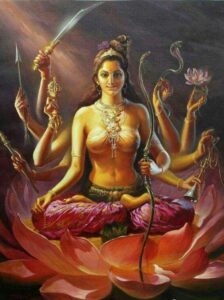
\includegraphics[width=.3\textwidth]{shakti-224x300.jpg}
\end{wrapfigure}

In the Tantric view of things, the world is the Play of Shakti, by which the ``divine Mother screens Herself in the form of interplaying Centres.'' But there is only one centre: ``The experience of the Supreme I is ``I am the Universe. The limited I identifies himself with a particular mind and body in it.'' So how do we Play? Are there rules? Can we improve our game?

In a sport---let's take golf as an example---it is elementary. The rules are known in advance and it is a simple matter to count the number of strokes to hole the ball. There can be no possible dispute about best player on a given day. This is why sports appeals to the masses. Even when they play themselves, they accept their inferiority to the top players in the game. So how to reach the top?

Performance experts say it takes about 10,000 hours of practice, whether of a sport or musical instrument, to reach the very peak of talent, and 7500 may get you close. However, the top golfers will be out hitting balls for hours at a time. Besides the talent itself, at a certain level, there is honour to the game. A golfer won't kick the ball out of the rough and he will report even unseen transgressions of the rules.

So how do we then excel at our game, that is, the game of Joy and Free Power, that veils the Supreme I in a kaleidoscope of multiplicity? Well, let's look at an example. We know that Evola studied the corpus of 19th century German Idealism, along with many other contemporary thinkers. He made himself conversant in Oriental philosophies: early Buddhism, Tantra, Taoism. To this he added a vast familiarity with the range of European history and the mythology of the world. And just as a golfer would not rely on books but would go hit several buckets of balls, so, too, did Evola engage in spiritual exercises to peal away the veils of Shakti.

This commitment is what we must aspire to. The conceit that spending five minutes reading a post is sufficient to come to a sound judgment is risible, and those commenters that do so, just bring shame on themselves.

Every game has its starting position and ours is the vantage point of the limited I, which forgets he is playing and defends his own perspective or point of view, as though it were Absolute truth. Yet, to begin playing we first must understand that

\begin{quotex}
The entire universe of sensations, feelings, ideas, memories, and so forth, which constitute total Experience at any moment, can never be thought about as a whole ... Perfect Experience is thus alogical. Although unthinkable and indescribable, it is not on that account unknown and unknowable. It is Experience itself, Consciousness itself.
\end{quotex}


Hence, at some point, thought must be abandoned, in favour of the ``Supreme Intuition''. This is why, for example, the man who has experience of Spirit and Soul in his consciousness is not confused about their relationship. This is why the man who has experience of the states of being understands the nature of caste distinctions, and so on.

\begin{quotex}
The only reality is Consciousness, a position for which we may argue but which cannot be established with certitude except by an actual or direct experience of unity. Those who seek to establish supersensible truths on any other ground must fail; just as those who argue against the validity of the individual's experience must fail.
\end{quotex}


So here is another way to improve our game:

\begin{quotex}
Mind reveals Consciousness by degrees, some minds more than the rest. The purer the mind the more it reflects or manifests Consciousness. The object then of the self-realising discipline or Sadhana is to purify the Mind so that it may manifest Consciousness. Purity of Mind is therefore to be sought... It is obvious that if a Mind is dominated by sensuous desires and images, it cannot reflect or show Spirit.
\end{quotex}


Besides the purification of the Mind, it must also be developed:

\begin{quotex}
The Mind must be an efficient and trained instrument of knowledge which is its appropriate food, and should if necessary be sharpened by the study of logic and the practice of debate.
\end{quotex}


Reality is Logos, so a sane and rational mind is mandatory, but also a well-bred mind.

\begin{quotex}
Philosophising is not done because of mere intellectual curiosity but as part of a disciplinary system enjoined for the realization by the limited self of its own unlimited and essential nature. That nature has its intellectual aspect and is expressed as Reason. For what is irrational cannot be spiritually true.
\end{quotex}

All unattributed quotations are from \emph{The World as Power} by John Woodroffe.


\flrightit{Posted on 2011-03-22 by Cologero}

